\documentclass[]{article}
\usepackage{lmodern}
\usepackage{amssymb,amsmath}
\usepackage{ifxetex,ifluatex}
\usepackage{fixltx2e} % provides \textsubscript
\ifnum 0\ifxetex 1\fi\ifluatex 1\fi=0 % if pdftex
  \usepackage[T1]{fontenc}
  \usepackage[utf8]{inputenc}
\else % if luatex or xelatex
  \ifxetex
    \usepackage{mathspec}
  \else
    \usepackage{fontspec}
  \fi
  \defaultfontfeatures{Ligatures=TeX,Scale=MatchLowercase}
\fi
% use upquote if available, for straight quotes in verbatim environments
\IfFileExists{upquote.sty}{\usepackage{upquote}}{}
% use microtype if available
\IfFileExists{microtype.sty}{%
\usepackage{microtype}
\UseMicrotypeSet[protrusion]{basicmath} % disable protrusion for tt fonts
}{}
\usepackage[margin=1in]{geometry}
\usepackage{hyperref}
\hypersetup{unicode=true,
            pdftitle={Bright Spots and Blind Spots},
            pdfborder={0 0 0},
            breaklinks=true}
\urlstyle{same}  % don't use monospace font for urls
\usepackage{graphicx,grffile}
\makeatletter
\def\maxwidth{\ifdim\Gin@nat@width>\linewidth\linewidth\else\Gin@nat@width\fi}
\def\maxheight{\ifdim\Gin@nat@height>\textheight\textheight\else\Gin@nat@height\fi}
\makeatother
% Scale images if necessary, so that they will not overflow the page
% margins by default, and it is still possible to overwrite the defaults
% using explicit options in \includegraphics[width, height, ...]{}
\setkeys{Gin}{width=\maxwidth,height=\maxheight,keepaspectratio}
\IfFileExists{parskip.sty}{%
\usepackage{parskip}
}{% else
\setlength{\parindent}{0pt}
\setlength{\parskip}{6pt plus 2pt minus 1pt}
}
\setlength{\emergencystretch}{3em}  % prevent overfull lines
\providecommand{\tightlist}{%
  \setlength{\itemsep}{0pt}\setlength{\parskip}{0pt}}
\setcounter{secnumdepth}{0}
% Redefines (sub)paragraphs to behave more like sections
\ifx\paragraph\undefined\else
\let\oldparagraph\paragraph
\renewcommand{\paragraph}[1]{\oldparagraph{#1}\mbox{}}
\fi
\ifx\subparagraph\undefined\else
\let\oldsubparagraph\subparagraph
\renewcommand{\subparagraph}[1]{\oldsubparagraph{#1}\mbox{}}
\fi

%%% Use protect on footnotes to avoid problems with footnotes in titles
\let\rmarkdownfootnote\footnote%
\def\footnote{\protect\rmarkdownfootnote}

%%% Change title format to be more compact
\usepackage{titling}

% Create subtitle command for use in maketitle
\providecommand{\subtitle}[1]{
  \posttitle{
    \begin{center}\large#1\end{center}
    }
}

\setlength{\droptitle}{-2em}

  \title{Bright Spots and Blind Spots}
    \pretitle{\vspace{\droptitle}\centering\huge}
  \posttitle{\par}
  \subtitle{A kick-ass project}
  \author{}
    \preauthor{}\postauthor{}
      \predate{\centering\large\emph}
  \postdate{\par}
    \date{23 February 2020}


\begin{document}
\maketitle

\hypertarget{abstract}{%
\section{Abstract}\label{abstract}}

\hypertarget{main-text}{%
\section{Main Text}\label{main-text}}

\hypertarget{intro}{%
\subsection{Intro}\label{intro}}

The famous Blue Marble photograph taken by the crew of Apollo 17
embodies the abundance of water that supported the emergence of life on
Earth and is intrinsically linked to human health, ecosystem function,
and economic prosperity. Yet, this iconic picture belies the pressures
facing freshwater resources today, brought about by anthropogenic
threats of human population growth and urbanization (Jenerette and
Larsen 2006; Immerzeel et al. 2020), climate variability and change
(Gosling and Arnell 2016), economic growth and consumption patterns
(Mcdonald et al. 2014; O'dorico et al. 2018), and the spread of
misinformation and mistrust in science (IPCC 2014). To support societal
and ecological water needs in this context, decision-making must be
based on evidence from robust water resources research in a diversity of
scientific fields (Uzzi et al. 2013). A typical combinations and
scientific impact, which spans spatial (Zipper et al. 2020) and temporal
scales of resource management, and is connected by collaborations within
and across countries and disciplines (Astudillo 2016). This definition
of robust research can be used to identify bright and blind spots of
past scientific inquiry, that is topics and locations where water issues
are more- or less-thoroughly understood, respectively (Cvitanovic and
Hobday 2018).

Latin America embodies these water challenges with its unequal
distribution of abundant water resources for a small population (DESA
2019), mounting pollution and the highest income inequality in the world
(Varis, Taka, and Kummu 2019). Marked disparities between and within
countries affect water resources management, such as water supply,
climate change vulnerability, urbanization level, habits and scientific
productivity (Ciocca and Delgado 2017; Lyon et al. 2019). Countries with
abundant surface water resources, such as Brazil, experience water
scarcity due to a mismatch between water-ich areas and population
centers (Formiga-Johnsson and Kemper, n.d.), while others face flooding
and melting glaciers, such as Argentina, Chile and Bolivia (Barros et
al. 2015; Soruco et al. 2015; Masiokas et al. 2019). Latin America is
among the most urbanized regions in the world and these high density
areas face particular vulnerability to water quality and supply risks
(Kim and Grafakos 2019). The city of Sāo Paulo nearly ran out of water
during a 2014 drought, while Mexico City is steadily and rapidly
depleting its groundwater supply (Aguilar-Barajas et al. 2015). Urban
pressures on water resources are compounded by poor farming practices,
unregulated industries, and aging infrastructure across the region.
These water challenges are expected to intensify due to climate change
as variations in precipitation, temperature, and evaporation threaten
water availability for current and future water users around the globe,
and particularly in Latin America (Dussaillant et al. 2019; Garreaud et
al. 2017; Gesualdo et al. 2019; Zaninelli et al. 2019). Uncertainty
surrounds the reliability of water supplies to meet future needs as well
as the availability of funds for scientific research to address future
water scarcity (Andrade 2019).

\hypertarget{challenge}{%
\subsection{Challenge}\label{challenge}}

Given these circumstances, it is critical to assess whether water
resources research across Latin America contributes the knowledge
necessary to successfully manage water.

While others did\ldots\ldots\ldots{} there are shortcomings.

To assess the state of this research, we performed an unprecedented,
multi-lingual review of the state of water resources research literature
in the region and across a range of topics and disciplines. This
literature review reveals bright spots and blind spots of past water
research and provides insights for scientists and decision-makers to
advance the relevance and impact of future scientific inquiries and to
design effective policy solutions to resource management challenges.

\hypertarget{action}{%
\subsection{Action}\label{action}}

Our two-fold, novel and comprehensive research approach combines
advanced computation with a stakeholder survey to describe past water
research in Latin America. First, we performed a data-driven literature
review by assembling a corpus of 30,000 water resources research
articles and analyzing them with a topic model. We used Latent Dirichlet
Allocation (LDA, (Blei, Ng, and Jordan 2003)), a generative Bayesian
model, which describes topics as a probability distribution over words
and documents as a probability distribution over topics. Human reading
validated the document topics and identified the country of study of
2,000 articles. Combined with article metadata and text mining, this
information was used to predict the country of study across the corpus
with machine learning. In-corpus citing and cited references were used
to build a citation network which, combined with topic and location
information, infers connectivity between research communities.

Second, to understand the landscape of water research in Latin America,
we collected publicly available data and conducted an on line survey.
Countries within Latin America were statistically clustered into four
groups with distinct physiographic and socioeconomic characteristics. To
ground our data-driven results in the reality of the current research
climate, we invited nearly 20,000 corresponding authors to share their
experiences through a survey focused on research discipline,
accessibility and connectivity.

A chord diagram describes the composition of water research in Latin
America and the Caribbean and reveals inequalities in locations and
themes of research (figure 1). The chord widths indicate the proportion
of a specific research theme within the top 25\% of research for a given
country. While Brazil, Mexico, Argentina and Chile dominate the research
landscape, countries the Caribbean and most of Central American are
excluded from the analysis, indicating a relative shortage of research
in these regions. A country's socio-economic cluster correlates to its
contribution to overall research output, which suggests that a country's
resources, geography and history influence its scientific activity.
Similarly, water research is not distributed equally among disciplines
and results from our corpus reveal a relative shortage of research in
the social sciences. While Mexico contributes most to the social science
research, it is a small proportion of its overall output. Water research
is conducted primarily in the physical and life sciences, with Mexico
and Argentina alternating for second highest output after Brazil,
respectively.

After assessing trends in the corpus, we further analyzed results from
the topic model and text mining to identify bright spots and blind spots
of water research in Latin America and the Caribbean. We define
successful research as having a distributions that is normally and with
high entropy. When applied to our corpus, these concepts highlight
locations and themes that are relatively under-researched.

Water research in Latin America and the Caribbean has generally higher
normality across countries than documents (figure 2). A look at the
normalities of the components of the water budget validates our analysis
approach. Rivers and precipitation, which must be monitored and
understood to manage water resources, have distributions closest to
normal, while glaciers are far from normally distribution because few
countries have glaciers to study. This analysis clearly identifies the
main research methods that are used in water research, which include
spatial methods, statistics, quantitative methods and water sampling.
Following the decreasing gradient of normality points next to the niche
topics, such as irrigation and isotopes, which have high normality
across countries but low normality across documents. These values
indicate that topics in this region of the graph are not often discussed
with other research topics or included in interdisciplinary papers. The
least normality is seen in two topics of great importance for water
management: reservoirs and risk assessment.

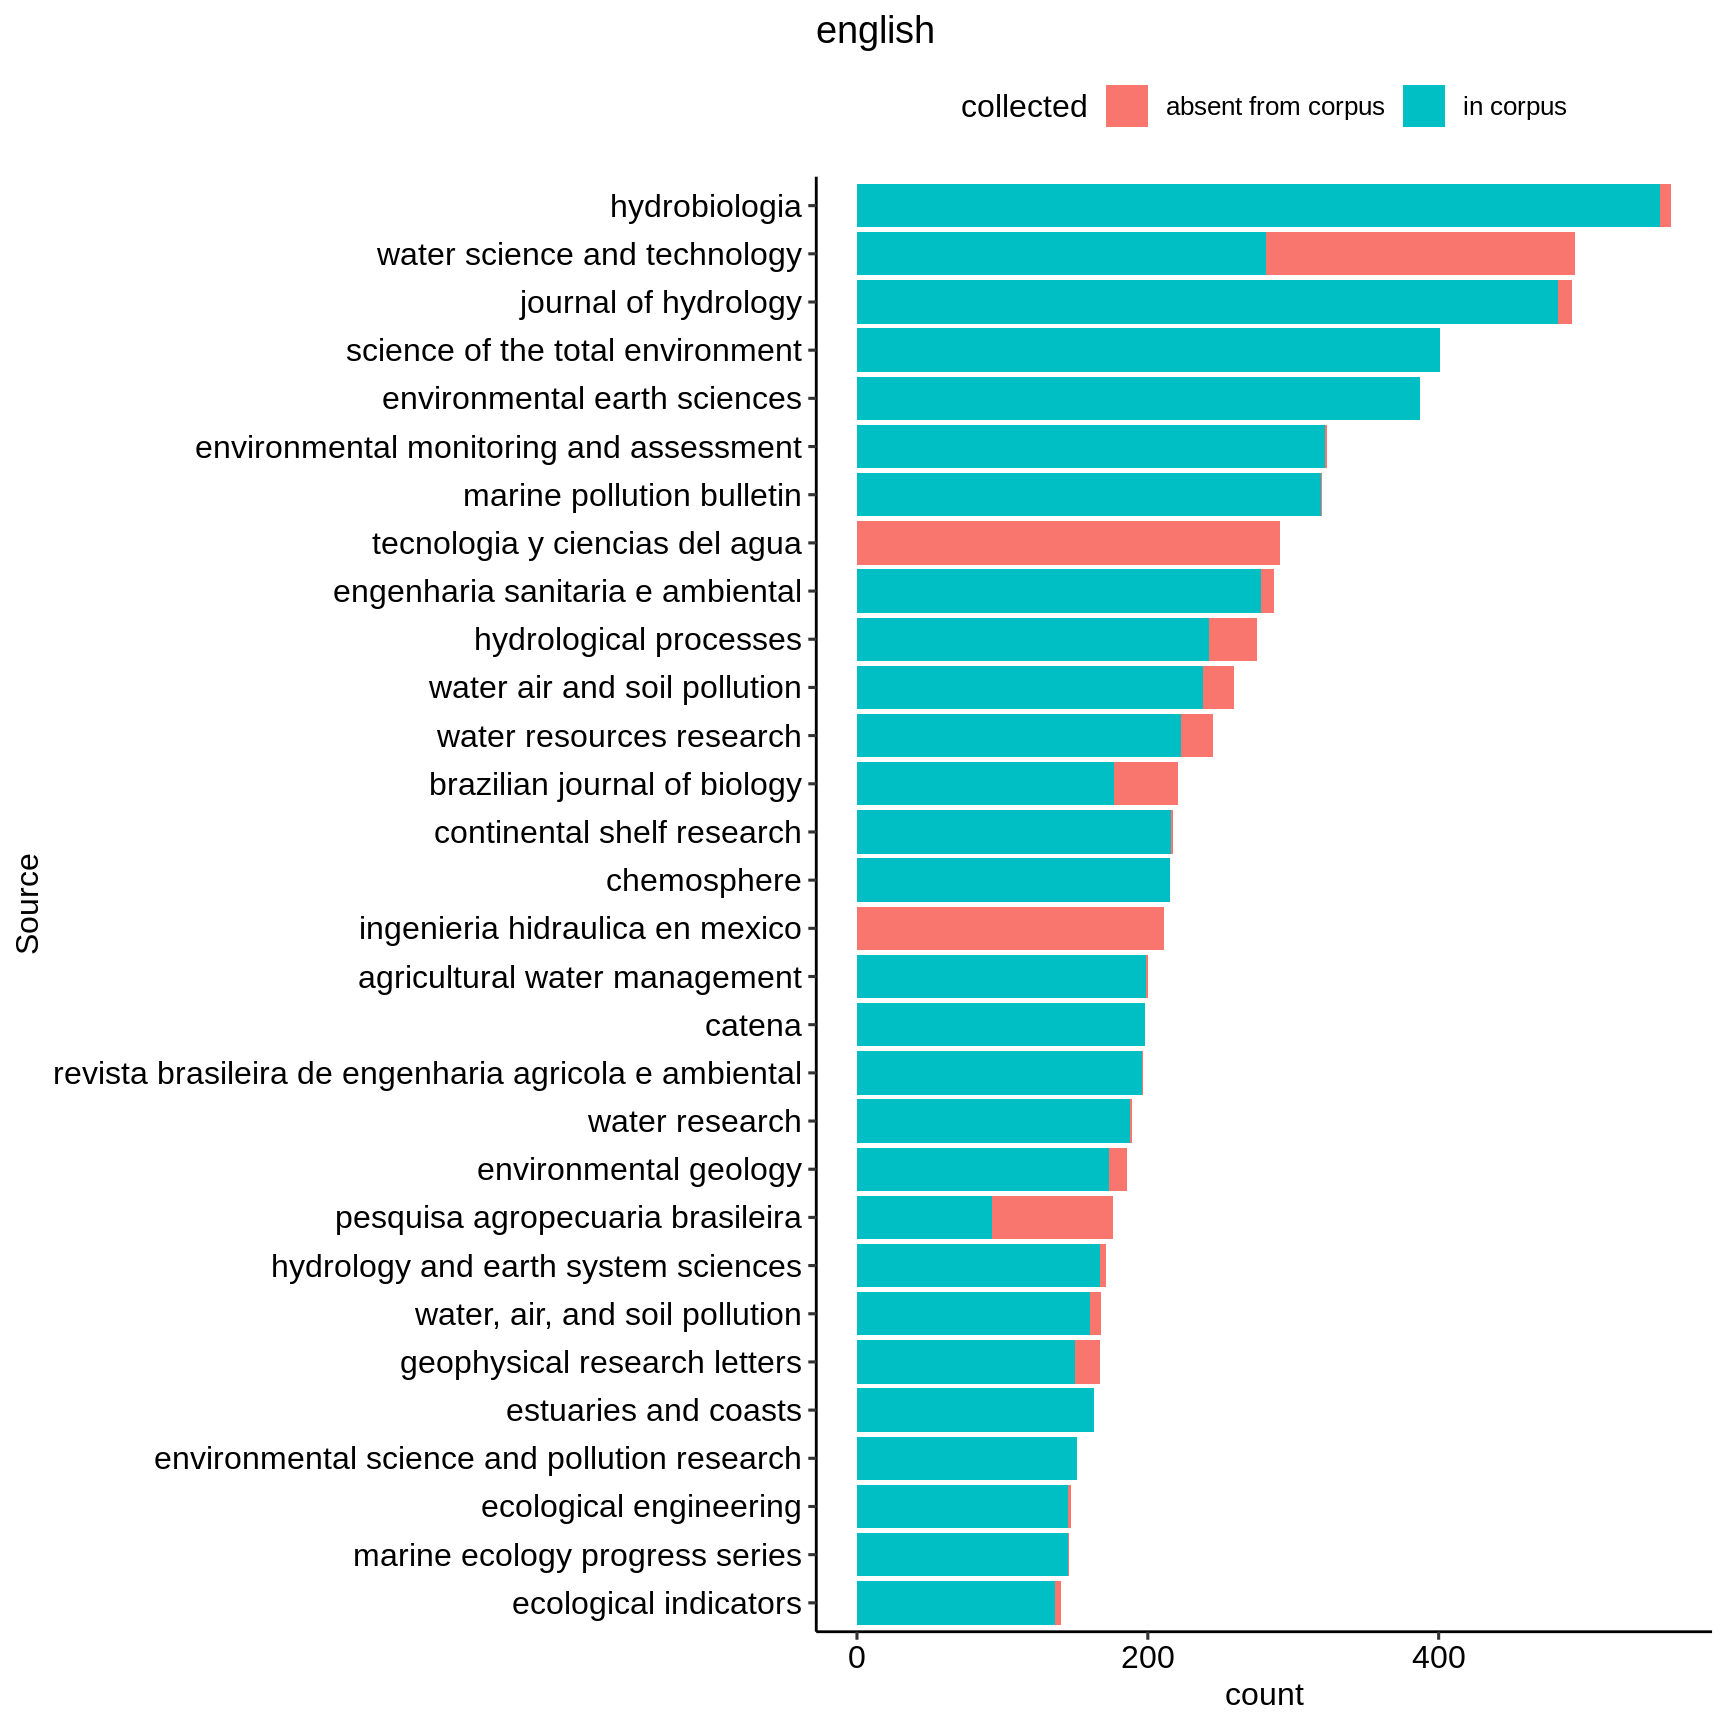
\includegraphics{article_files/figure-latex/unnamed-chunk-6-1.pdf}

\begin{center}\rule{0.5\linewidth}{\linethickness}\end{center}

\hypertarget{references}{%
\section*{References}\label{references}}
\addcontentsline{toc}{section}{References}

\hypertarget{refs}{}
\leavevmode\hypertarget{ref-Aguilar2015}{}%
Aguilar-Barajas, Ismael, Jürgen Mahlknecht, Jonathan Kaledin, Marianne
Kjellén, and Abel Mejı́a-Betancourt. 2015. \emph{Water and Cities in
Latin America: Challenges for Sustainable Development}. Routledge.

\leavevmode\hypertarget{ref-Andrade2019}{}%
Andrade, Rodrigo de Oliveira. 2019. ``Brazil Budget Cuts Threaten 80,000
Science Scholarships.'' NATURE PUBLISHING GROUP MACMILLAN BUILDING, 4
CRINAN ST, LONDON N1 9XW, ENGLAND.

\leavevmode\hypertarget{ref-Astudillo2016}{}%
Astudillo, Pablo. 2016. ``Manifesto for Science.'' \emph{Editorial:
CATALONIA-Fundaci ~'o N Science ~\& Life Collection ó N: Science ~\&
Life}.

\leavevmode\hypertarget{ref-Barros2015}{}%
Barros, Vicente Ricardo, José Armando Boninsegna, Inés Angela Camilloni,
Martina Chidiak, Graciela Odilia Magrı́n, and Matilde Rusticucci. 2015.
``Climate Change in Argentina: Trends, Projections, Impacts and
Adaptation.'' \emph{Wiley Interdisciplinary Reviews: Climate Change} 6
(2): 151--69.

\leavevmode\hypertarget{ref-Blei2003}{}%
Blei, David M, Andrew Y Ng, and Michael I Jordan. 2003. ``Latent
Dirichlet Allocation.'' \emph{Journal of Machine Learning Research} 3
(Jan): 993--1022.

\leavevmode\hypertarget{ref-Ciocca2017}{}%
Ciocca, Daniel R., and Gabriela Delgado. 2017. ``The Reality of
Scientific Research in Latin America; an Insider's Perspective.''
\emph{Cell Stress and Chaperones} 22 (6): 847--52.
\url{https://doi.org/10.1007/s12192-017-0815-8}.

\leavevmode\hypertarget{ref-Cvitanovic2018}{}%
Cvitanovic, Christopher, and Alistair J Hobday. 2018. ``Building
Optimism at the Environmental Science-Policy-Practice Interface Through
the Study of Bright Spots.'' \emph{Nature Communications} 9 (1): 3466.

\leavevmode\hypertarget{ref-desa2019united}{}%
DESA, UN. 2019. ``United Nations, Department of Economic and Social
Affairs, Population Division. World Population Prospects 2019:
Highlights.''

\leavevmode\hypertarget{ref-Dussaillant2019}{}%
Dussaillant, I, E Berthier, F Brun, M Masiokas, R Hugonnet, V Favier, A
Rabatel, P Pitte, and L Ruiz. 2019. ``Two Decades of Glacier Mass Loss
Along the Andes.'' \emph{Nature Geoscience} 12 (10): 802--8.

\leavevmode\hypertarget{ref-Formiga2005}{}%
Formiga-Johnsson, RM, and KE Kemper. n.d. ``Institutional and Policy
Analysis of River Basin Management in the Alto-Tiete River Basin, Sao
Paulo, Brazil, the World Bank.'' \emph{Policy Research Working Paper}
3650.

\leavevmode\hypertarget{ref-Garreaud2017}{}%
Garreaud, René D, Camila Alvarez-Garreton, Jonathan Barichivich, Juan
Pablo Boisier, Duncan Christie, Mauricio Galleguillos, Carlos LeQuesne,
James McPhee, and Mauricio Zambrano-Bigiarini. 2017. ``The 2010-2015
Megadrought in Central Chile: Impacts on Regional Hydroclimate and
Vegetation.'' \emph{Hydrology \& Earth System Sciences} 21 (12).

\leavevmode\hypertarget{ref-Gesualdo2019}{}%
Gesualdo, Gabriela Chiquito, Paulo Tarso Oliveira, Dulce Buchala Bicca
Rodrigues, and Hoshin Vijai Gupta. 2019. ``Assessing Water Security in
the São Paulo Metropolitan Region Under Projected Climate Change.''

\leavevmode\hypertarget{ref-Gosling2016}{}%
Gosling, Simon N, and Nigel W Arnell. 2016. ``A global assessment of the
impact of climate change on water scarcity,'' 371--85.
\url{https://doi.org/10.1007/s10584-013-0853-x}.

\leavevmode\hypertarget{ref-Immerzeel2019}{}%
Immerzeel, W W, A F Lutz, M Andrade, A Bahl, H Biemans, T Bolch, S Hyde,
et al. 2020. ``Importance and vulnerability of the world ' s water
towers.'' \emph{Nature} 577 (January).
\url{https://doi.org/10.1038/s41586-019-1822-y}.

\leavevmode\hypertarget{ref-IPCC2014}{}%
IPCC. 2014. ``Climate Change 2014: Synthesis Report. Contribution of
Working Groups I, Ii, and Iii to the Fifth Assessmetn Report of the
Intergovernmental Panel on Climate Change.'' Geneva, Switzerland: IPCC.

\leavevmode\hypertarget{ref-Jenerette2006}{}%
Jenerette, G Darrel, and Larissa Larsen. 2006. ``A Global Perspective on
Changing Sustainable Urban Water Supplies.'' \emph{Global and Planetary
Change} 50 (3-4): 202--11.

\leavevmode\hypertarget{ref-Kim2019}{}%
Kim, Hyejung, and Stelios Grafakos. 2019. ``Which Are the Factors
Influencing the Integration of Mitigation and Adaptation in Climate
Change Plans in Latin American Cities?'' \emph{Environmental Research
Letters} 14 (10): 105008.

\leavevmode\hypertarget{ref-Lyon2019}{}%
Lyon, Steve W, Peter Goethals, Petra Schneider, Luis Dominguez-Granda,
Henrietta Hampel, Norris Lam, Indira Nolivos, et al. 2019. ``Improving
Water Management Education Across the Latin America and Caribbean
Region.'' \emph{Water} 11 (11): 2318.

\leavevmode\hypertarget{ref-Masiokas2019}{}%
Masiokas, MH, L Cara, R Villalba, P Pitte, BH Luckman, E Toum, DA
Christie, C Le Quesne, and S Mauget. 2019. ``Streamflow Variations
Across the Andes (18--55 S) During the Instrumental Era.''
\emph{Scientific Reports} 9 (1): 1--13.

\leavevmode\hypertarget{ref-Mcdonald2014}{}%
Mcdonald, Robert I, Katherine Weber, Julie Padowski, Martina Flo,
Christof Schneider, Pamela A Green, Thomas Gleeson, et al. 2014. ``Water
on an urban planet : Urbanization and the reach of urban water
infrastructure'' 27: 96--105.
\url{https://doi.org/10.1016/j.gloenvcha.2014.04.022}.

\leavevmode\hypertarget{ref-Odorico2018}{}%
O'dorico, Paolo D, Kyle Frankel Davis, Lorenzo Rosa, Joel A Carr, Davide
Chiarelli, Jampel Dell Angelo, Jessica Gephart, et al. 2018. ``The
Global Food-Energy-Water Nexus.'' \emph{Reviews of Geophysics},
456--531. \url{https://doi.org/10.1029/2017RG000591}.

\leavevmode\hypertarget{ref-Soruco2015}{}%
Soruco, Alvaro, Christian Vincent, Antoine Rabatel, Bernard Francou,
Emmanuel Thibert, Jean Emmanuel Sicart, and Thomas Condom. 2015.
``Contribution of Glacier Runoff to Water Resources of La Paz City,
Bolivia (16 S).'' \emph{Annals of Glaciology} 56 (70): 147--54.

\leavevmode\hypertarget{ref-Uzzi2013}{}%
Uzzi, Brian, Satyam Mukherjee, Michael Stringer, and Ben Jones. 2013.
``Atypical Combinations and Scientific Impact,'' no. October: 468--73.

\leavevmode\hypertarget{ref-Varis2019}{}%
Varis, Olli, Maija Taka, and Matti Kummu. 2019. ``The Planet's Stressed
River Basins: Too Much Pressure or Too Little Adaptive Capacity?''
\emph{Earth's Future}.

\leavevmode\hypertarget{ref-Zaninelli2019}{}%
Zaninelli, Pablo G., Claudio G. Menéndez, Magdalena Falco, Noelia
López-Franca, and Andrea F. Carril. 2019. ``Future Hydroclimatological
Changes in South America Based on an Ensemble of Regional Climate
Models.'' \emph{Climate Dynamics} 52 (1): 819--30.
\url{https://doi.org/10.1007/s00382-018-4225-0}.

\leavevmode\hypertarget{ref-Zipper2020}{}%
Zipper, Samuel C, Fernando Jaramillo, Lan Wang Erlandsson, and Sarah E
Cornell. 2020. ``Integrating the Water Planetary Boundary With Water
Management From Local to Global Scales Earth ' s Future.''
\url{https://doi.org/10.1029/2019EF001377}.


\end{document}
